\documentclass{article}
\author{Juan David Villalobos}
\usepackage[utf8]{inputenc}
\date{20 de Julio de 2017}
\title{Tarea 3 Métodos Computacionales.}
\usepackage[utf8]{inputenc}
\usepackage{amsmath, amssymb, graphicx}
\usepackage[utf8]{inputenc}

\frenchspacing

\newcommand{\JournalIssue}[1]{%
		\hfill \textsc{20 de Julio de 2017}
		\par \normalsize \normalfont}

\newcommand{\NewsAuthor}[1]{%
			\hfill \textsc{Juan David Villalobos 201521143}
			\par \normalsize \normalfont}	
            
\newcommand{\JournalName}[1]{%
		\begin{center}	
			\Huge \usefont{T1}{m}{n}
			#1%
		\end{center}	
		\par \normalsize \normalfont}
        


\begin{document}
\JournalIssue{1}
\NewsAuthor{}
\JournalName{Tarea 3}

\section{Ecuación de Onda en 2D}

\begin{figure}[h!]
\centering
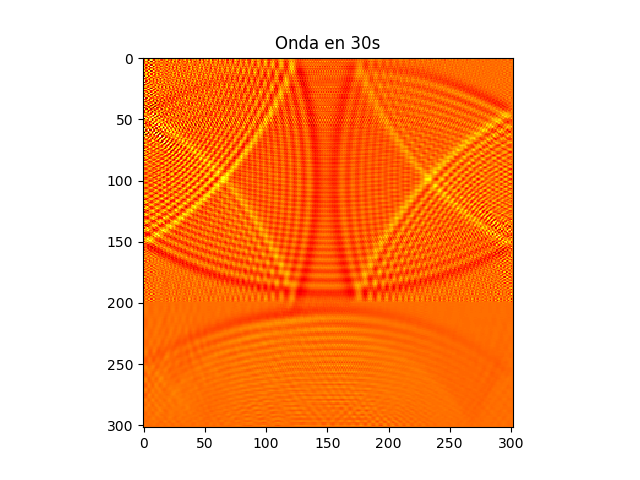
\includegraphics[width=0.7\textwidth]{tiempo=30s.png}
\caption{Desplazamiento de la onda 30 segundos despues de la perturbación}
\end{figure}

\begin{figure}[h!]
\centering
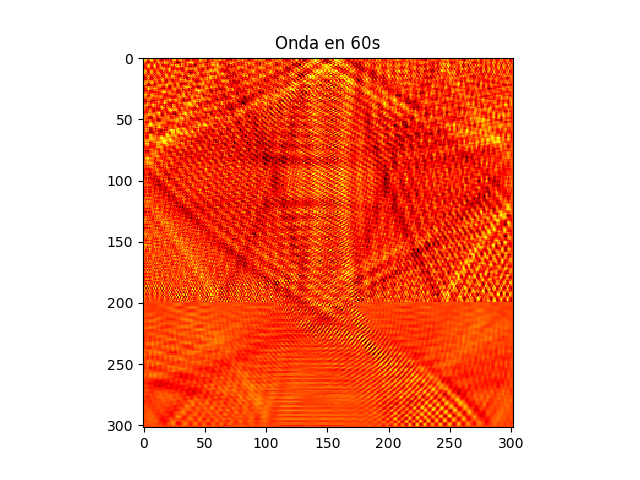
\includegraphics[width=0.7\textwidth]{tiempo=60s.png}
\caption{Desplazamiento de la onda 60 segundos despues de la perturbación}
\end{figure}

\section{Sistema solar}

\begin{figure}[h!]
\centering
\includegraphics[width=0.7\textwidth]{Orbitas.pdf}
\caption{Gráfica de las orbitas de los planetas}
\end{figure}


\end{document}
